\chapter{Diagramme}
Um sich diese Diagramme genauer ansehen zu können, müssen sie mit einem PDF-Reader
geöffnet werden, der eine Zoom-Funktion besitzt.
\section{Milestone 1}
\subsection{GANTT-Diagramm Milestone 1}
 \begin{figure}[h]
 		\centering
 		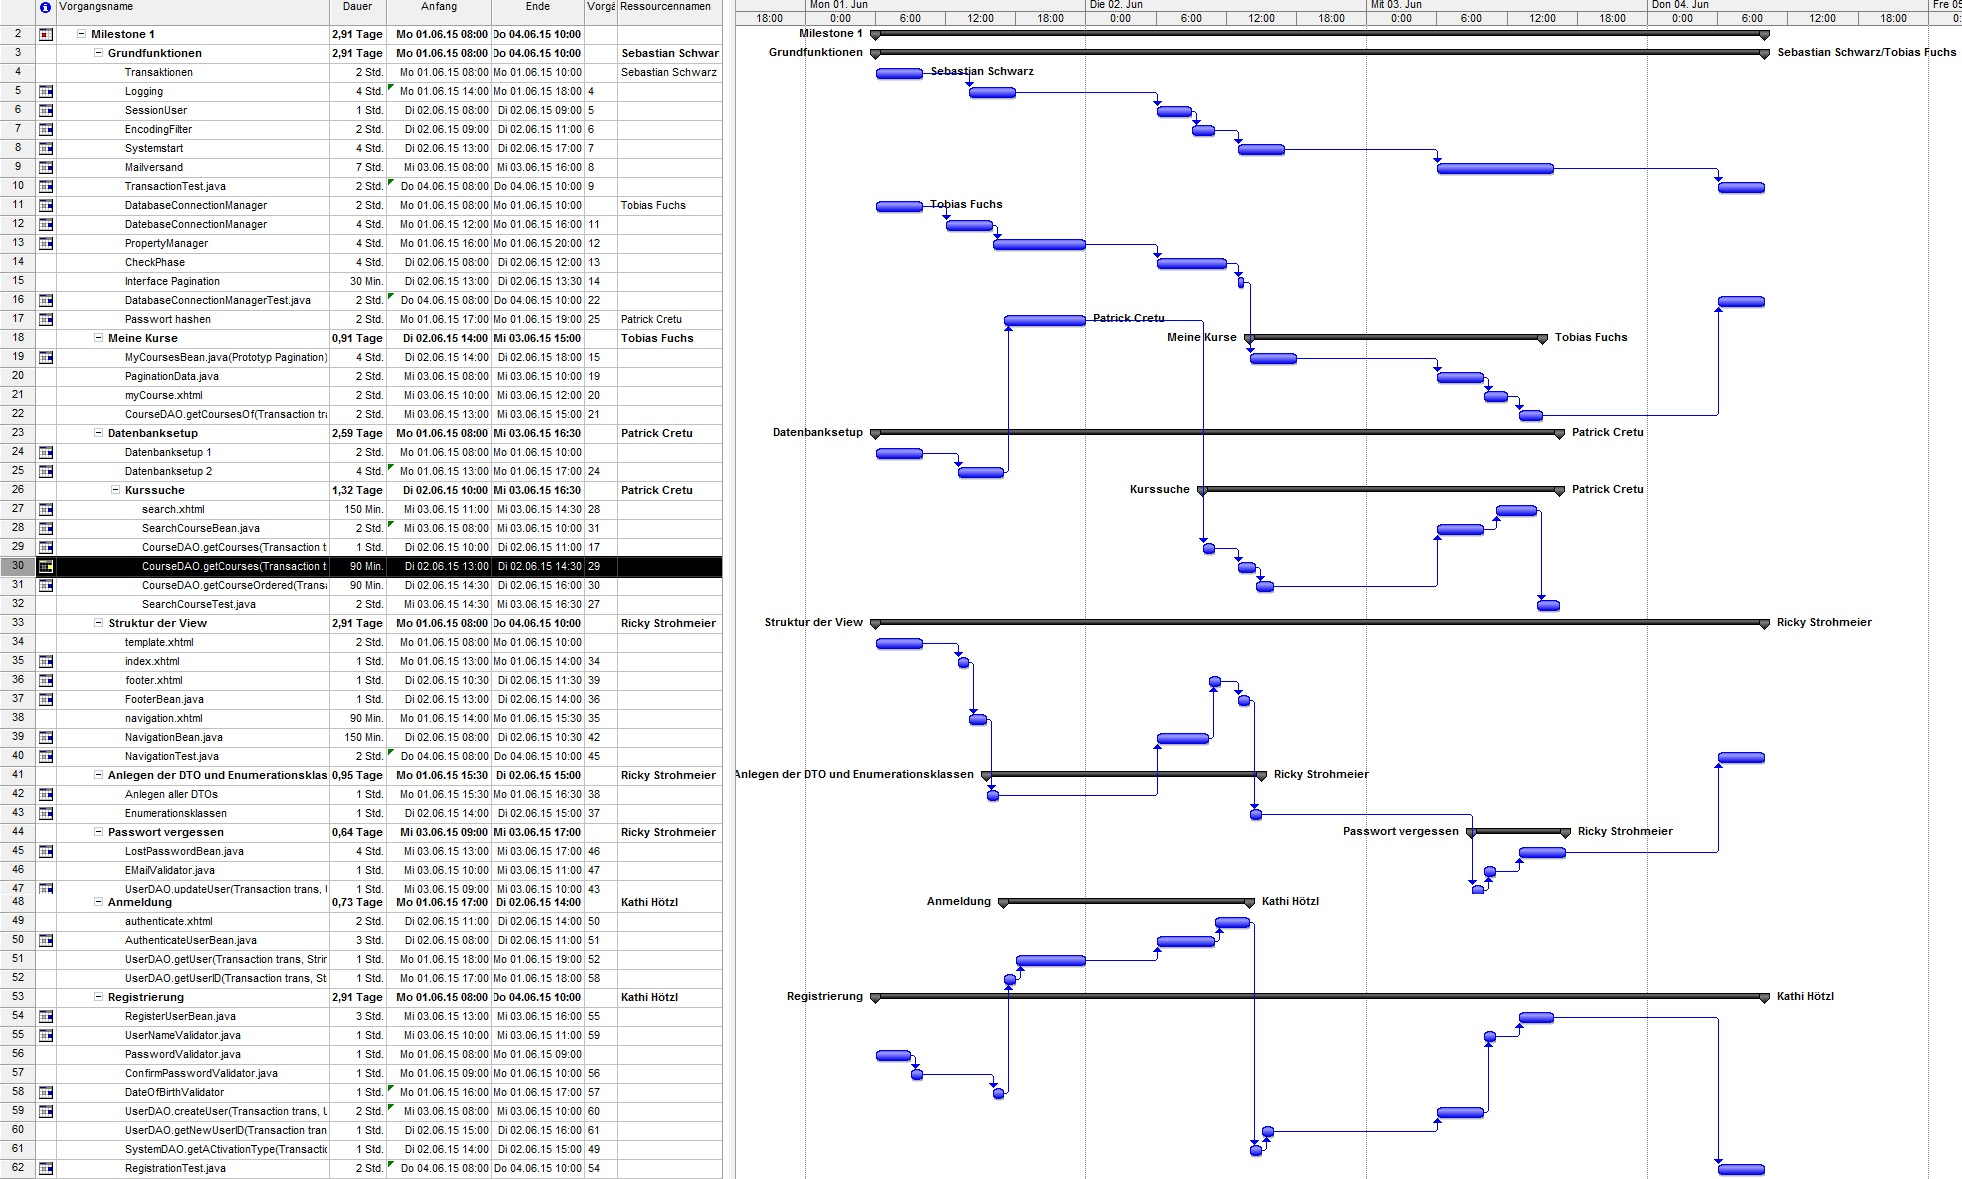
\includegraphics[width=0.8\linewidth, angle=90]{Grafiken/Milestone1Gantt}
 		\caption{GANTT-Diagramm Milestone 1}
 		\label{fig:GANTT-Diagramm Milestone 1}
 \end{figure}


\clearpage
\subsection{PERT-Diagramm Milestone 1}
\begin{figure}[h]
	\centering
	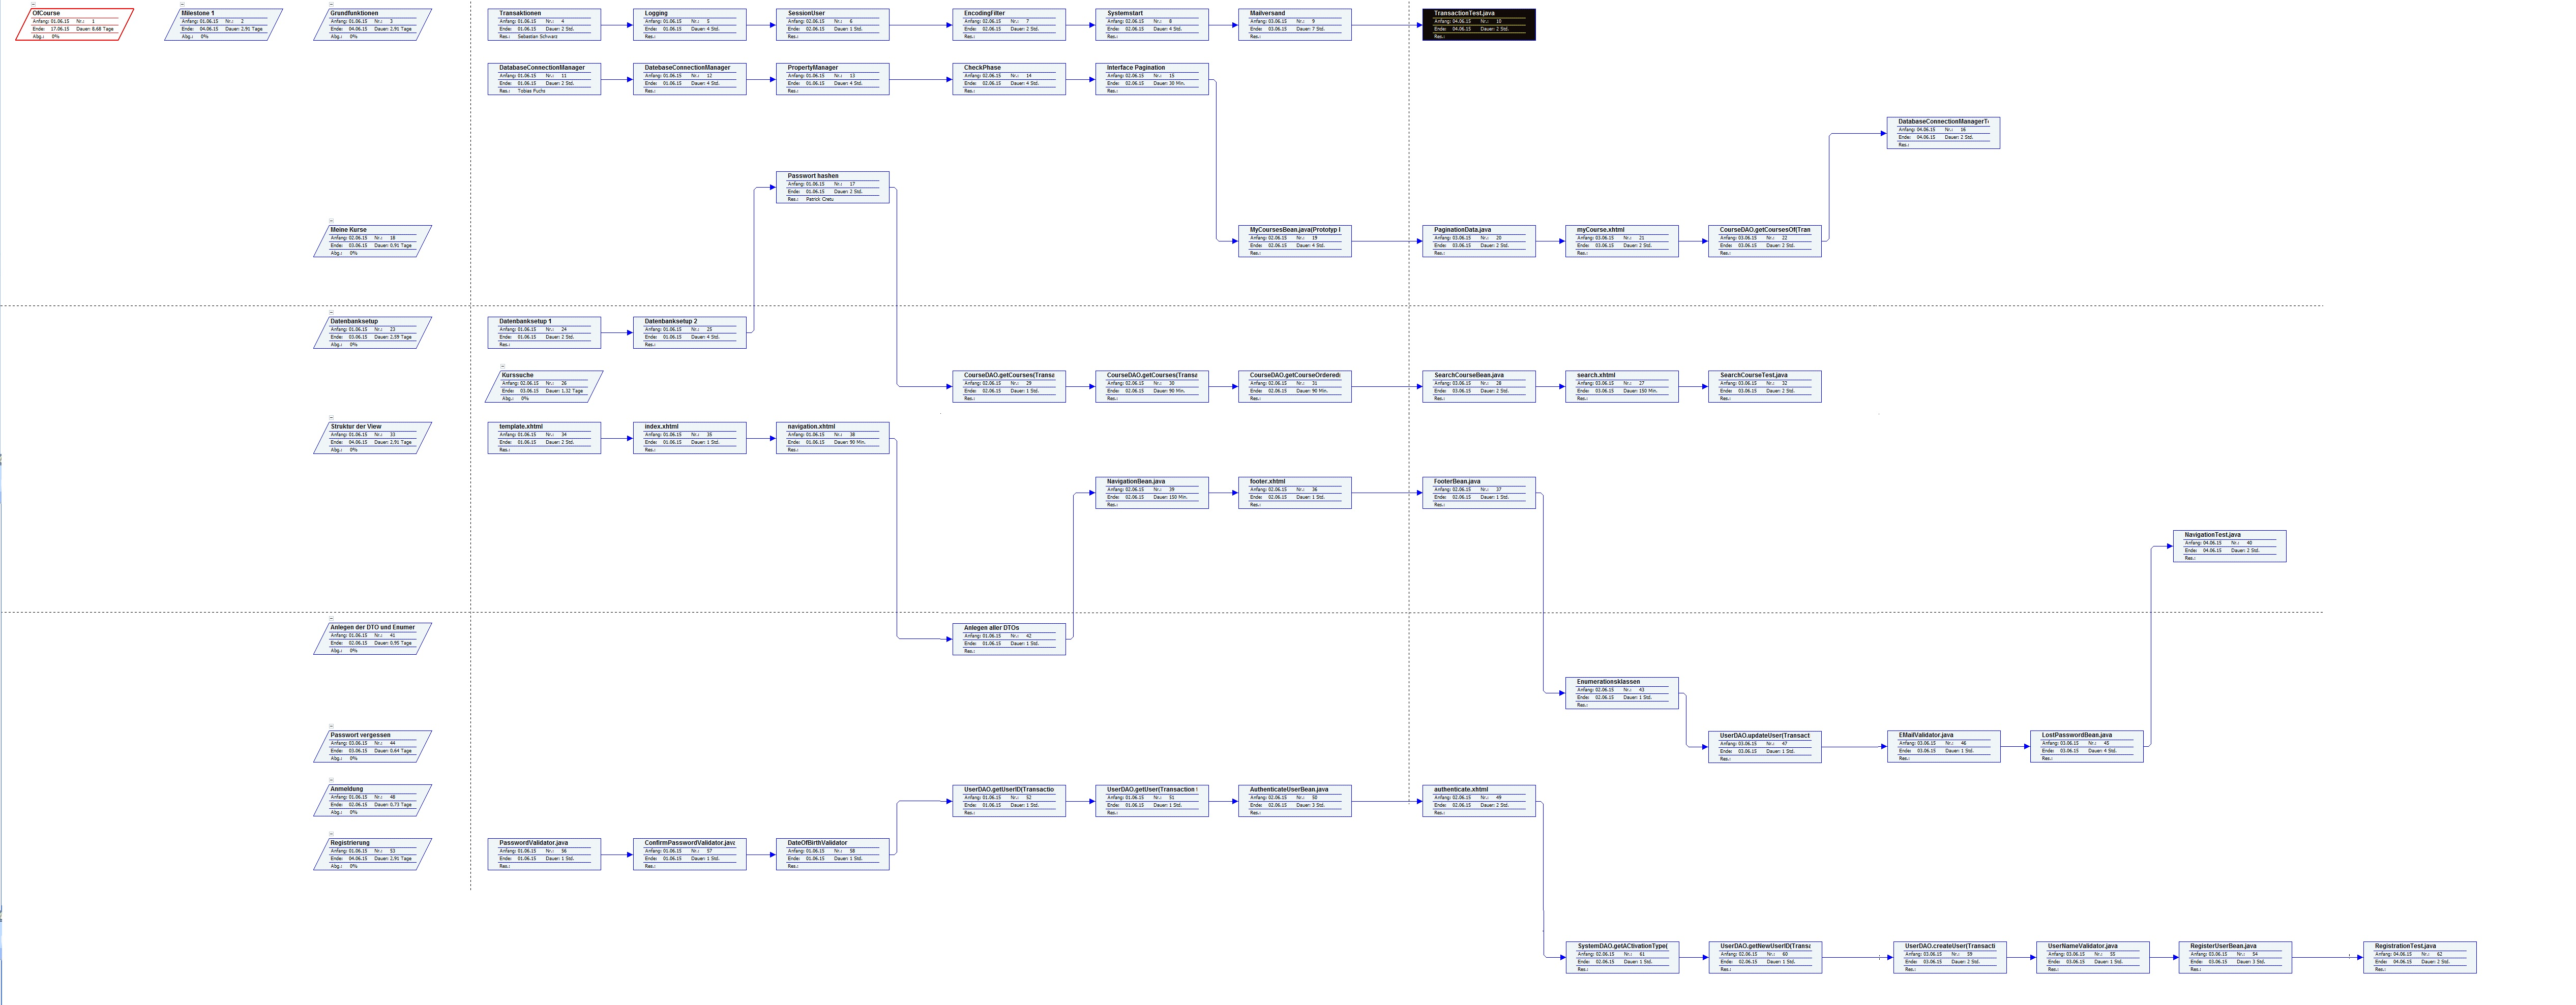
\includegraphics[width=1.0\linewidth, angle=90]{Grafiken/Milestone1Pert}
	\caption{PERT-Diagramm Milestone 1}
	\label{fig:PERT-Diagramm Milestone 1}
\end{figure}
\clearpage
\section{Milestone 2}
\subsection{GANTT-Diagramm Milestone 2}
\begin{figure}[h]
	\centering
	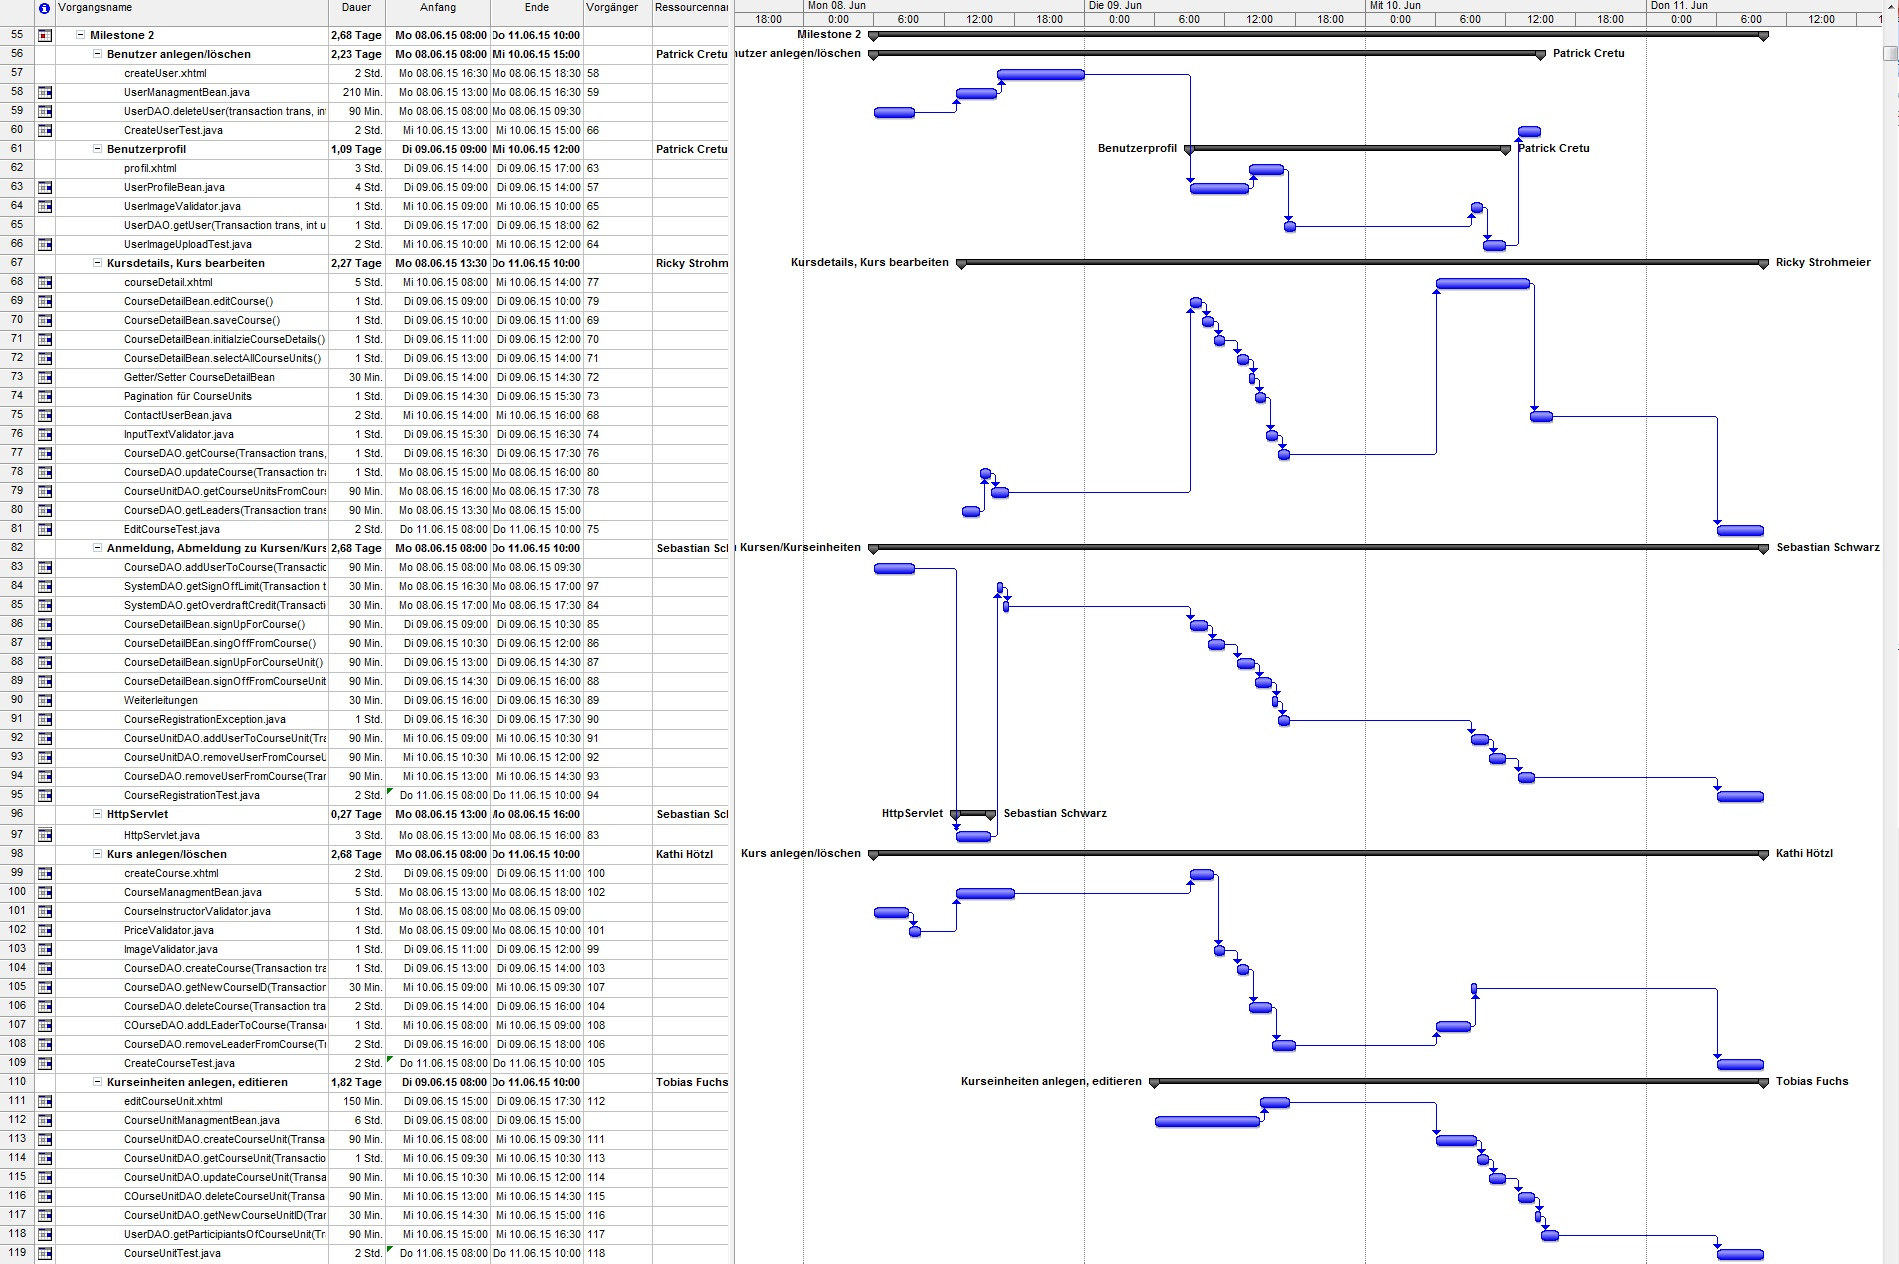
\includegraphics[width=1.0\linewidth, angle=90]{Grafiken/Milestone2Gantt}
	\caption{GANTT-Diagramm Milestone 2}
	\label{fig:GANTT-Diagramm Milestone 2}
\end{figure}

\clearpage
\subsection{PERT-Diagramm Milestone 2}
\begin{figure}[h]
	\centering
	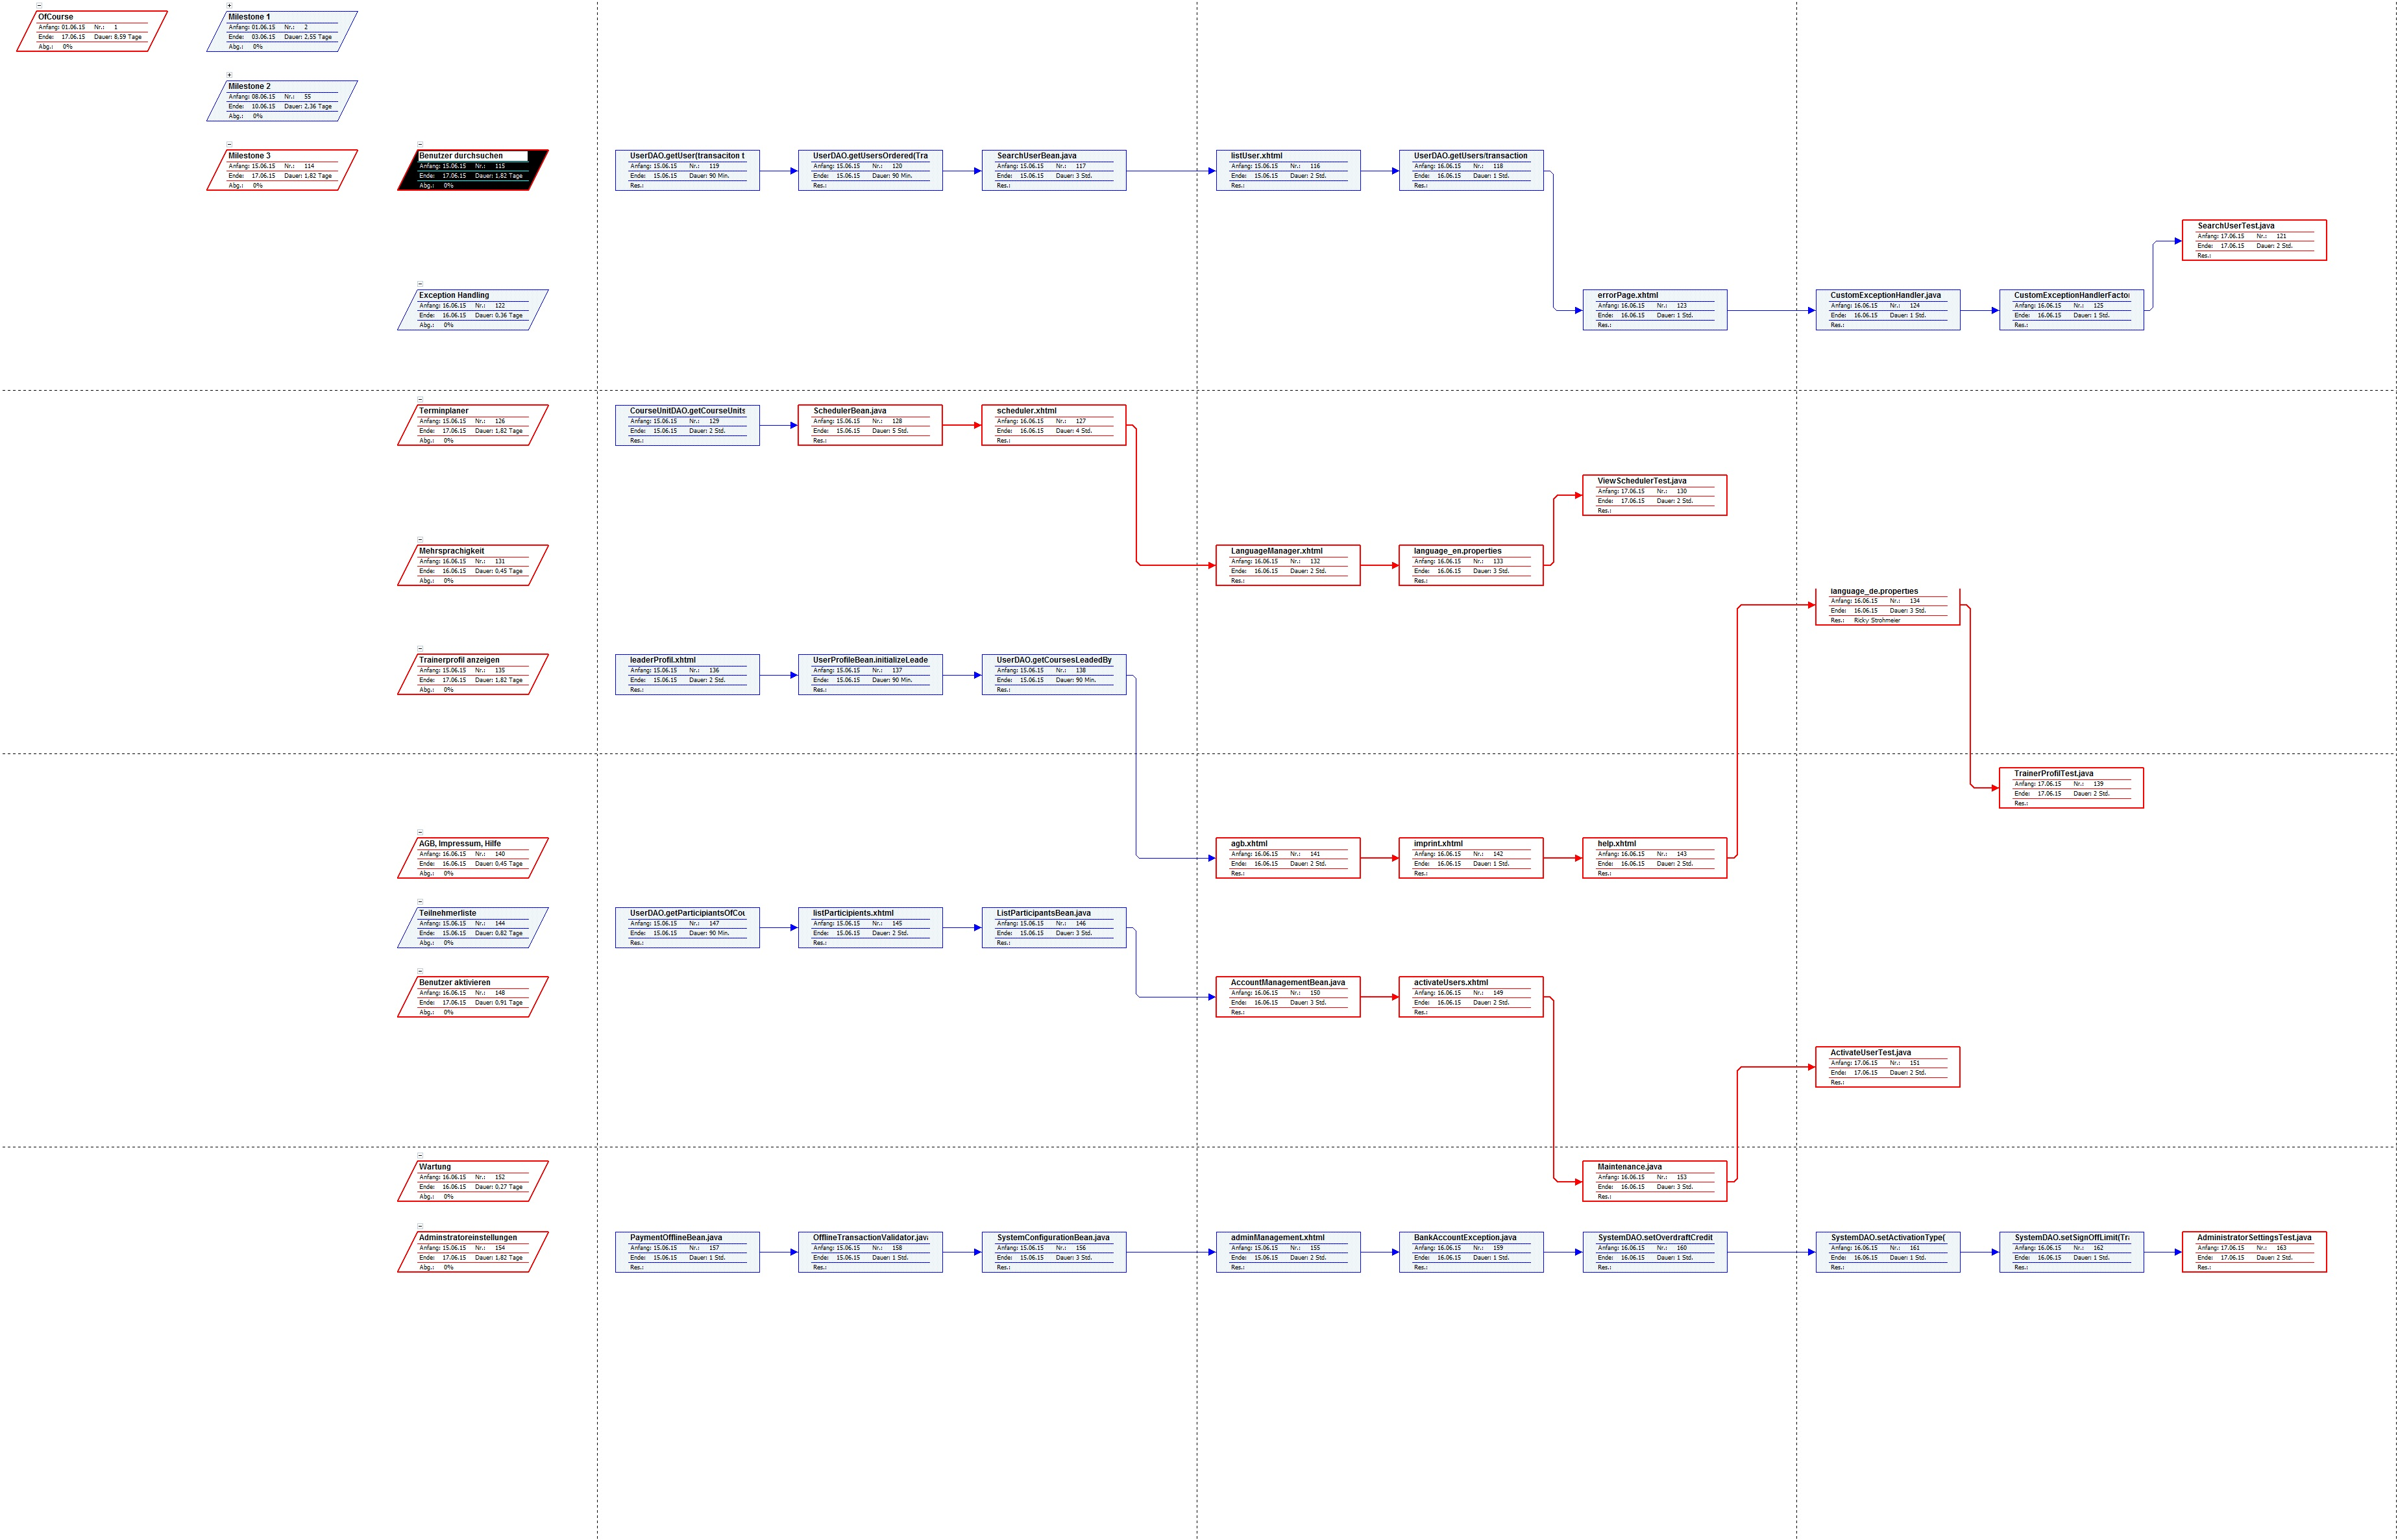
\includegraphics[width=1.0\linewidth, angle=90]{Grafiken/Milestone2Pert}
	\caption{PERT-Diagramm Milestone 2}
	\label{fig:PERT-Diagramm Milestone 2}
\end{figure}
\clearpage

\section{Milestone 3}
\subsection{GANTT-Diagramm Milestone 3}
\begin{figure}[h]
	\centering
	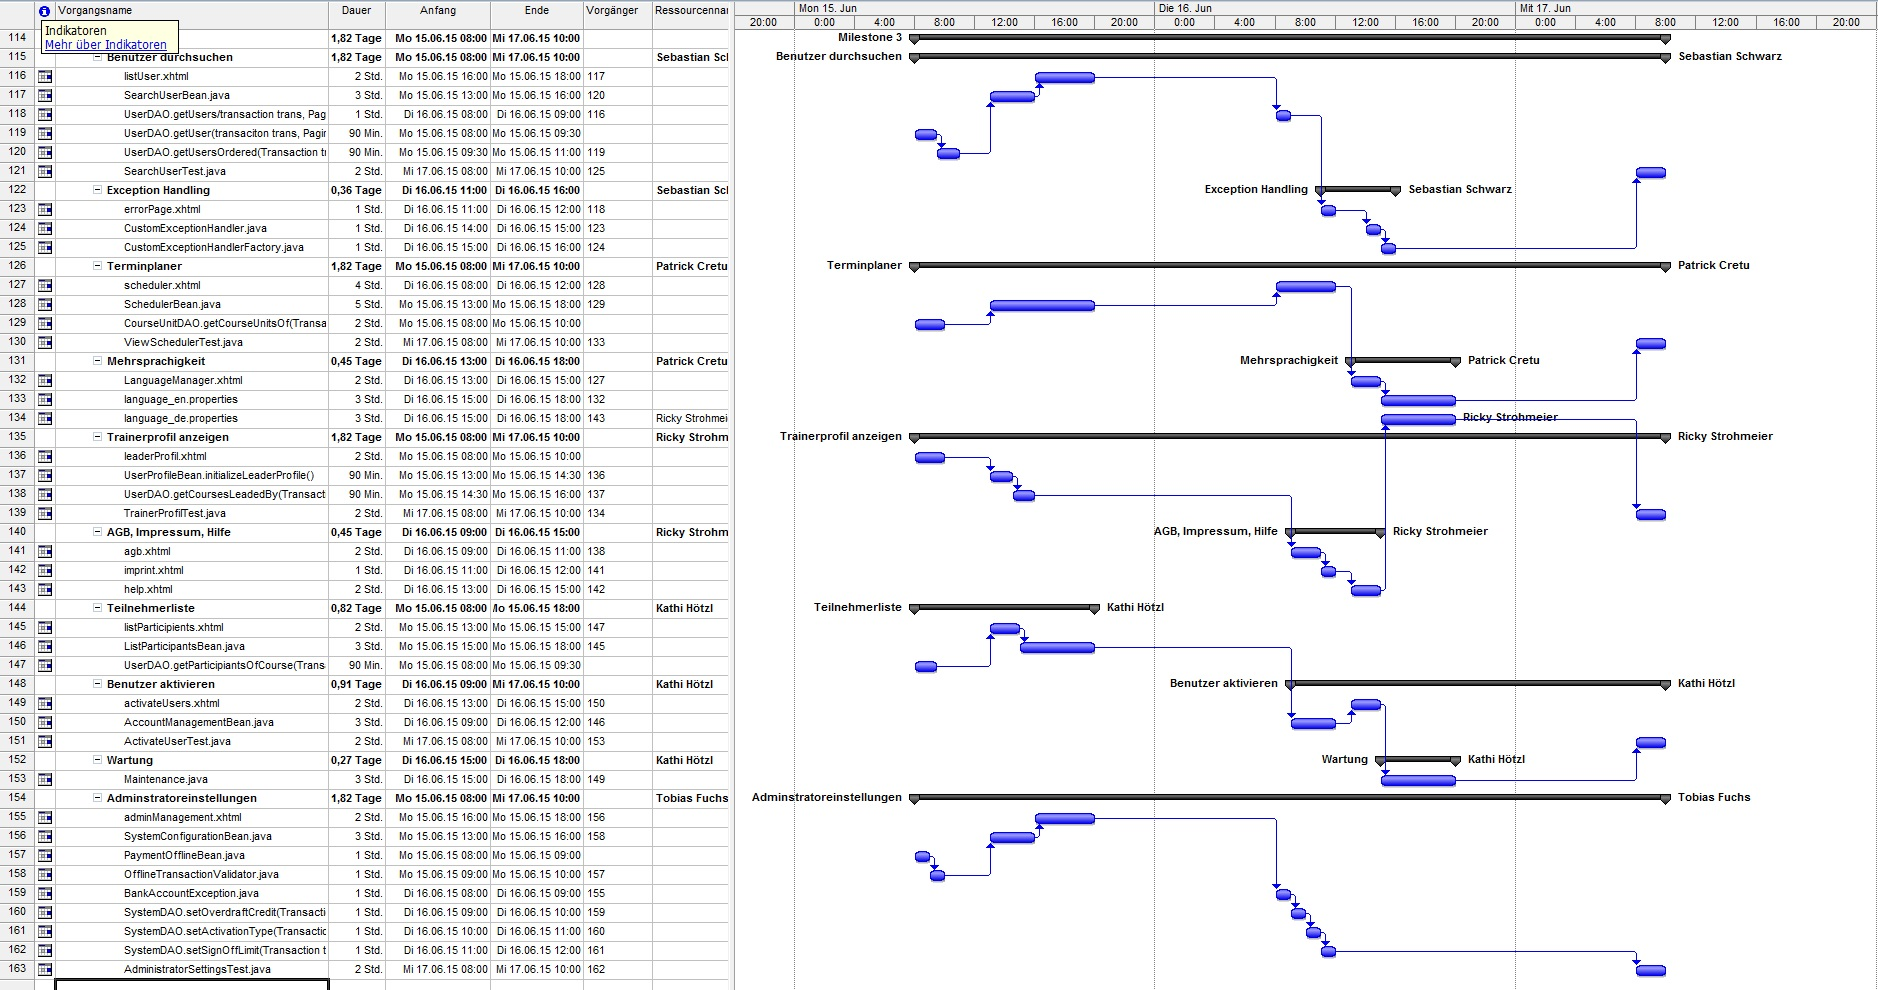
\includegraphics[width=1.0\linewidth, angle=90]{Grafiken/Milestone3Gantt}
	\caption{GANTT-Diagramm Milestone 3}
	\label{fig:GANTT-Diagramm Milestone 3}
\end{figure}
\clearpage

\subsection{PERT-Diagramm Milestone 3}
\begin{figure}[h]
	\centering
	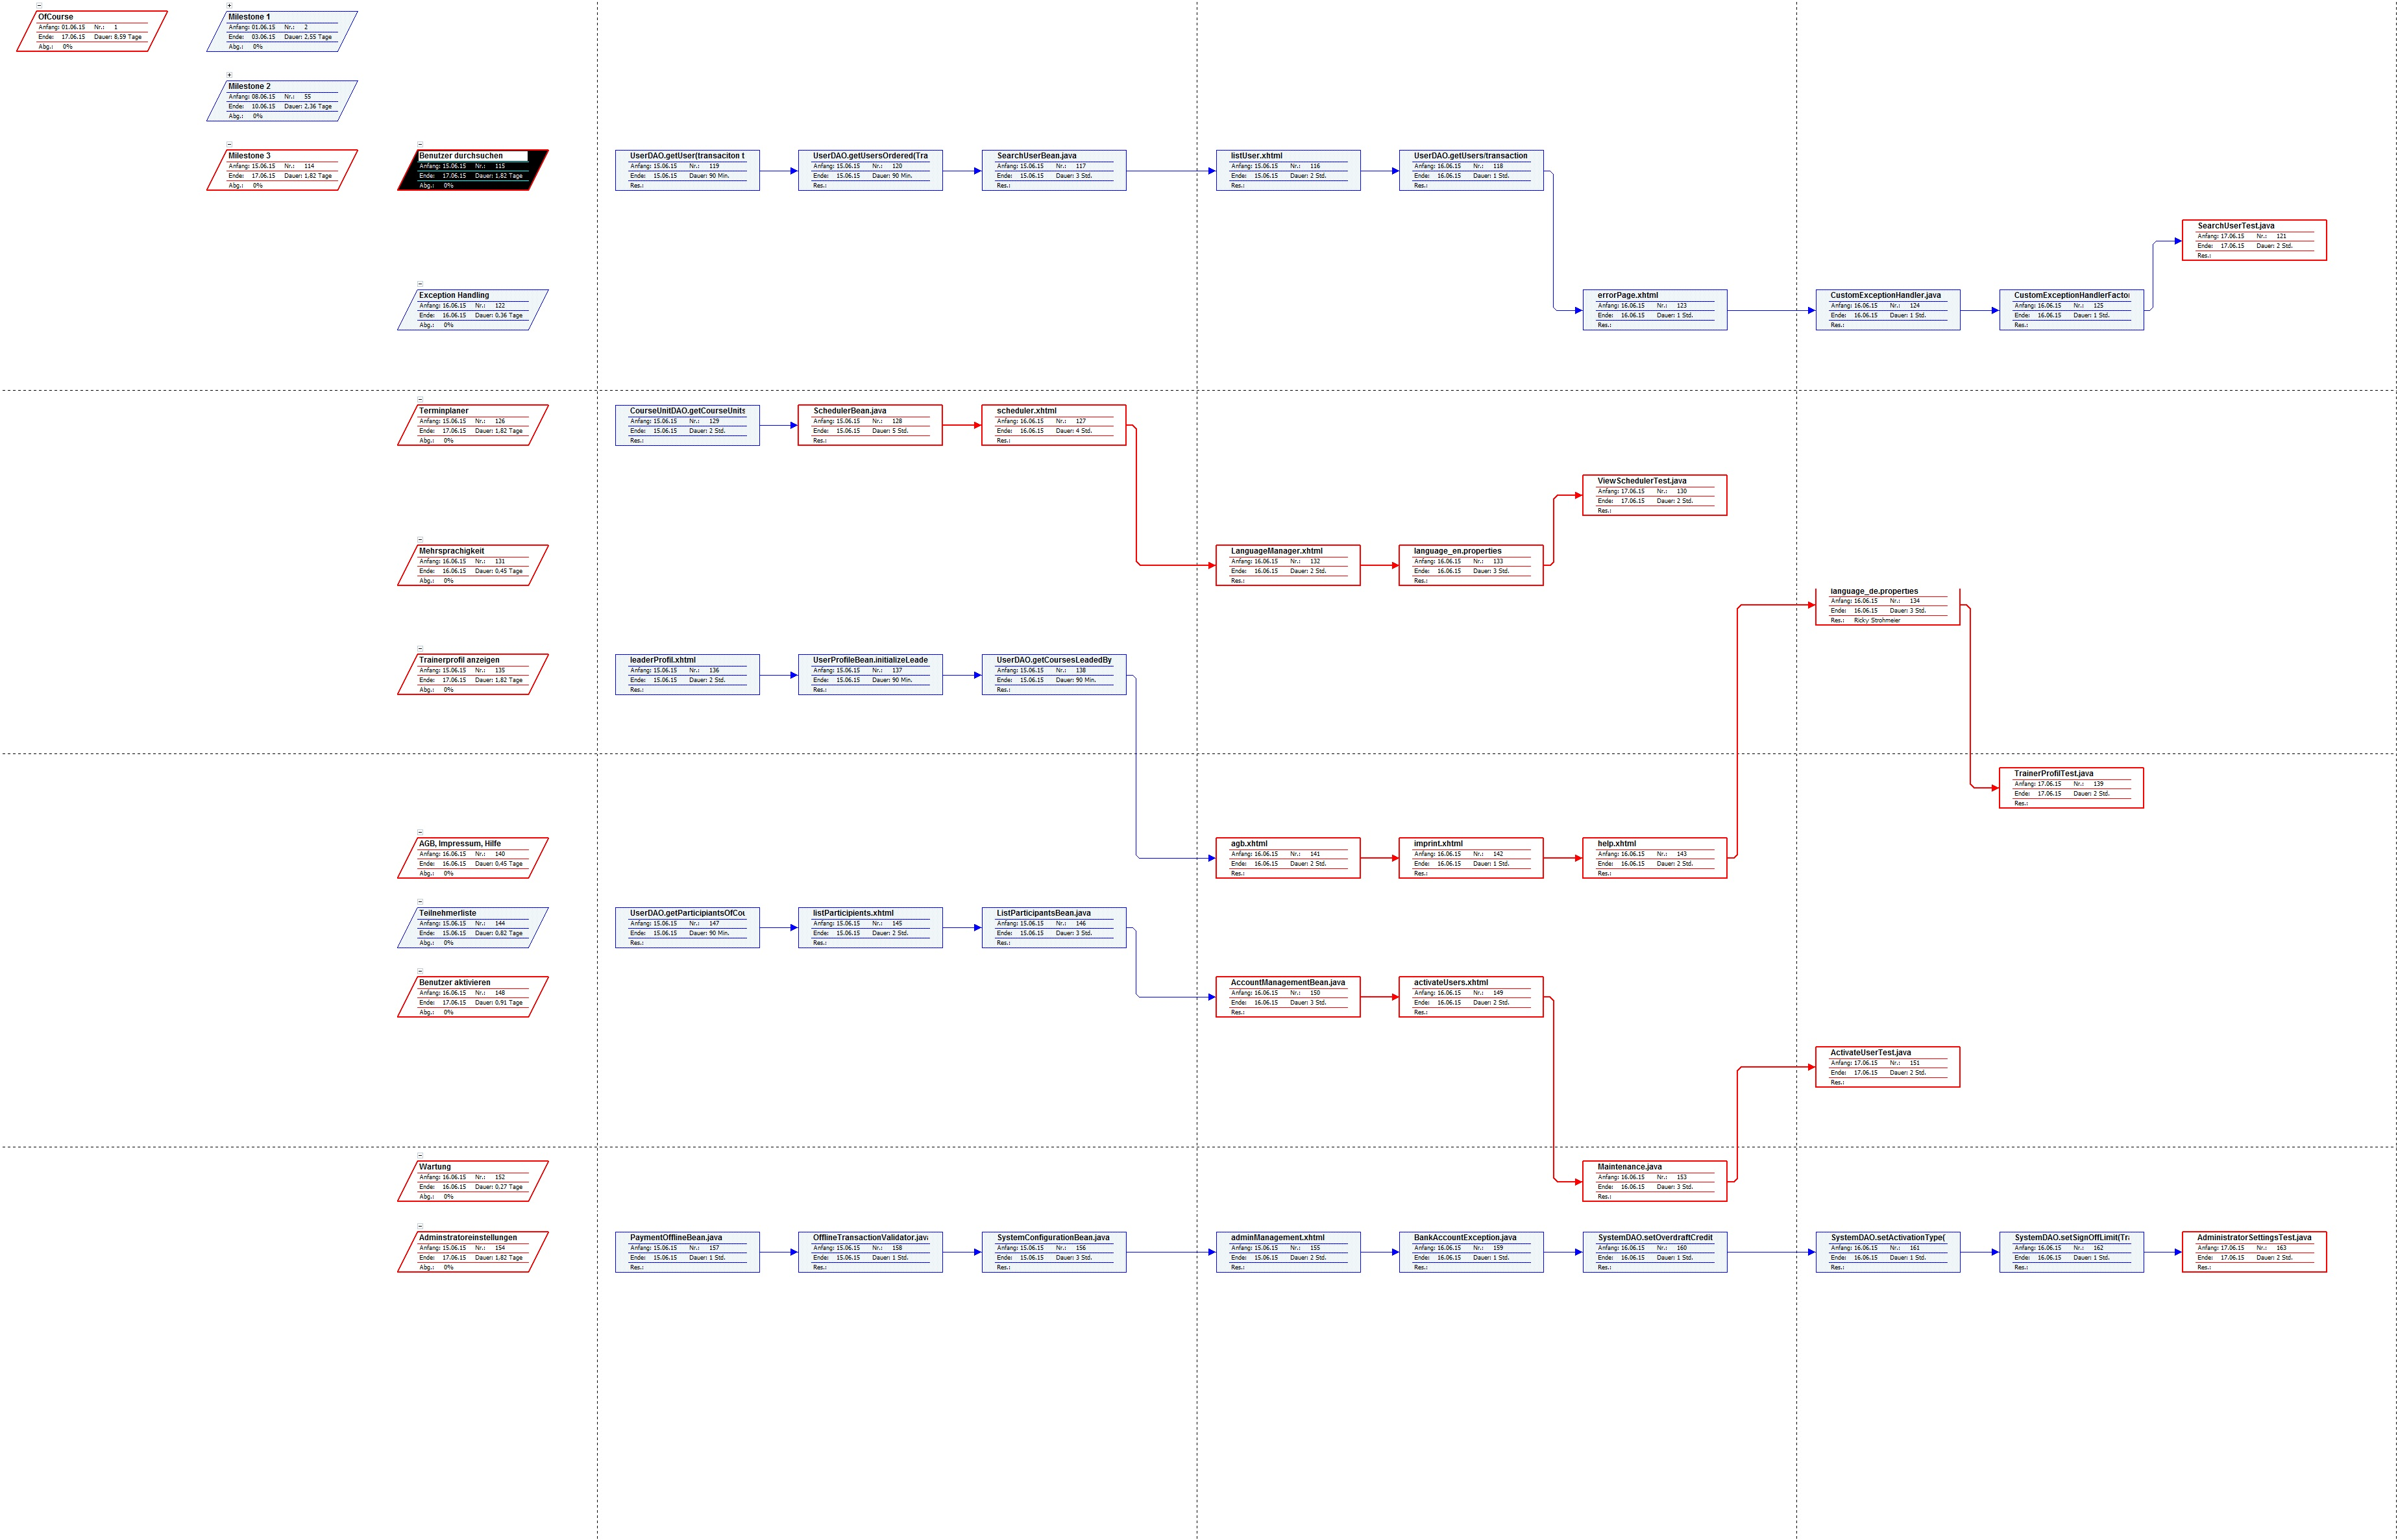
\includegraphics[width=1.0\linewidth, angle=90]{Grafiken/Milestone3PERT}
	\caption{PERT-Diagramm Milestone 3}
	\label{fig:PERT-Diagramm Milestone 3}
\end{figure}
\clearpage